% !TeX encoding   = UTF-8
\documentclass[12pt]{article}

\usepackage{sbc-template}

\usepackage{graphicx,url}
\usepackage[brazil]{babel}
\usepackage[utf8]{inputenc}
\usepackage{graphicx}	%Package para figuras
\usepackage{tabularx}
\usepackage{multirow} 
\usepackage[T1]{fontenc}
\usepackage{amsmath}
\usepackage{amsfonts}
\usepackage{amssymb}
\usepackage{makeidx}
\usepackage{graphicx}
\usepackage{lmodern}
\usepackage{epsfig}
\usepackage{adjustbox}
\usepackage{array}
\usepackage[linesnumbered,ruled,vlined]{algorithm2e}
\usepackage{enumerate}
\usepackage[table,xcdraw]{xcolor}
%\usepackage[left=2cm,right=2cm,top=2cm,bottom=2cm]{geometry}

     
\sloppy

\title{Projeto e Análise de Algoritmos\\ Trabalho Prático 2: \\
Identificando Ataques Sybil}

\author{Vagner Clementino\inst{1}}

\address{Departamento de Ciência da Computação\\
	   Universidade Federal de Minas Gerais (UFMG)\\  
  \email{vagnercs@dcc.ufmg.br}
}

\begin{document} 

\maketitle

%\begin{abstract}
%  This meta-paper describes the style to be used in articles and short papers
%  for SBC conferences. For papers in English, you should add just an abstract
%  while for the papers in Portuguese, we also ask for an abstract in
%  Portuguese (``resumo''). In both cases, abstracts should not have more than
%  10 lines and must be in the first page of the paper.
%\end{abstract}
     
%\begin{resumo} 
%TO DO
%\end{resumo}


\section{Introdução}
\label{sec:intro}

As \textit{redes sociais} vêm se mostrando um local propício para que os criminosos virtuais apliquem os seus golpes. Diversos tipos de atividades maliciosas, tais como \textit{spam}, \textit{phishing}, \textit{malware} e \textit{falsificação de perfis} são constantes ameaças aos usuários das redes. Um tipo de ameaça que vêm crescendo dentro das redes sociais é o ataque \textit{Sybil}. Nesse tipo de ameaça, usuários criam múltiplas identidades com o objetivo de criar relacionamentos sociais com usuários reais com finalidades maliciosas \cite{viswanath2011analysis}.

Em alto nível, todos mecanismos de defesa existentes tentam isolar vértices Sybil que estão incorporados dentro da topologia de uma rede social. Cada mecanismo determina se um vértice na rede ou é Sybil ou não-Sybil (honesto) da perspectiva de um vértice honesto efetivamente particionando os vértices da rede social em duas regiões distintas, a saber: região honesta e a região Sybil. Uma região honesta no grafo G é um subgrafo que consiste de todos os vértices honestos e arestas entre eles. Por sua vez, uma região Sybil, é composta por
vértices maliciosos e arestas entre eles. As arestas em G que conectam a região honesta com a região Sybil são chamadas de arestas de ataque, conforme é apresentado na Figura \ref{fig:sybil}.

\begin{figure}[ht]
\centering
\includegraphics[width=0.5\textwidth]{../img/sybil.png}
\caption{Região honesta e região Sybil.}
\label{fig:sybil}
\end{figure}

Este documento está organizado da seguinte forma: a Seção \ref{sec:solucao} descreve a solução proposta, detalhamento a modelagem do problema bem como o algoritmo para particionamento do grafo na região Sybil e Honesta; na Seção \ref{sec:analise_complexidade} é apresentado a análise de complexidade de tempo e espaço da algoritmo proposto; a Seção \ref{sec:experimentos} é devotada a análise experimental do algoritmo, tendo um foco especial no comportamento do mesmo para grafo de diferentes tipos utilizando para tal o conjunto de métricas descritos na Subseção \ref{subsec:metricas}; o documento é finalizado na Seção \ref{sec:conclusao} onde as conclusões obtidas são discutidas bem como as possíveis implicações dos resultados encontrados.

\section{Descrição da Solução}
\label{sec:solucao}
Esta Seção é devotada à explicação do algoritmo proposto para detecção de usuários \textit{Sybil}. Em suma, o algoritmo proposto recebe um grafo representado uma rede social e realiza o particionamento do mesmo em duas regiões, a região \emph{honesta (A)} e a região \emph{Sybil (B)}. Iniciemos detalhando a modelagem de grafo utilizada.

\subsection{Modelagem do Problema}
\label{subsec:modelagem}

Uma Rede Social pode ser modelada como um grafo $G = (V, E)$ \emph{não direcionado}. O conjunto $V$ é o conjunto de \textit{vértices}, em cada vértice representará um usuário da rede. De forma análoga, o conjunto $E$ é o conjunto de \textit{arestas}, e tem como objetivo representar um relacionamento social entre dois usuários da rede.

Tradicionalmente os grafos são modelados utilizando estruturas de dados tais como matriz ou lista de adjacência. Neste trabalho, contudo, utilizou-se uma representação um pouco diferente para um grafo. A estrutura de dados grafo foi representada como um conjunto de \textit{Vértices}. Estes, por sua vez, armazenam um conjunto de \textit{Arestas}, as quais armazenam os vértices inicial e final em que a aresta é incidente. A Figura \ref{fig:cd_graph} exibe um diagrama de classe UML\cite{rumbaugh2004unified}{}. A principal vantagem desta modelagem está em sua flexibilidade tendo em vista que é possível construir facilmente tanto grafos direcionados quanto não direcionados. Ademais, este tipo de representação facilidade bastante o processo de remoção ou adição de arestas ou vértices ao grafo durante a execução do algoritmo.

\begin{figure}[ht]
\centering
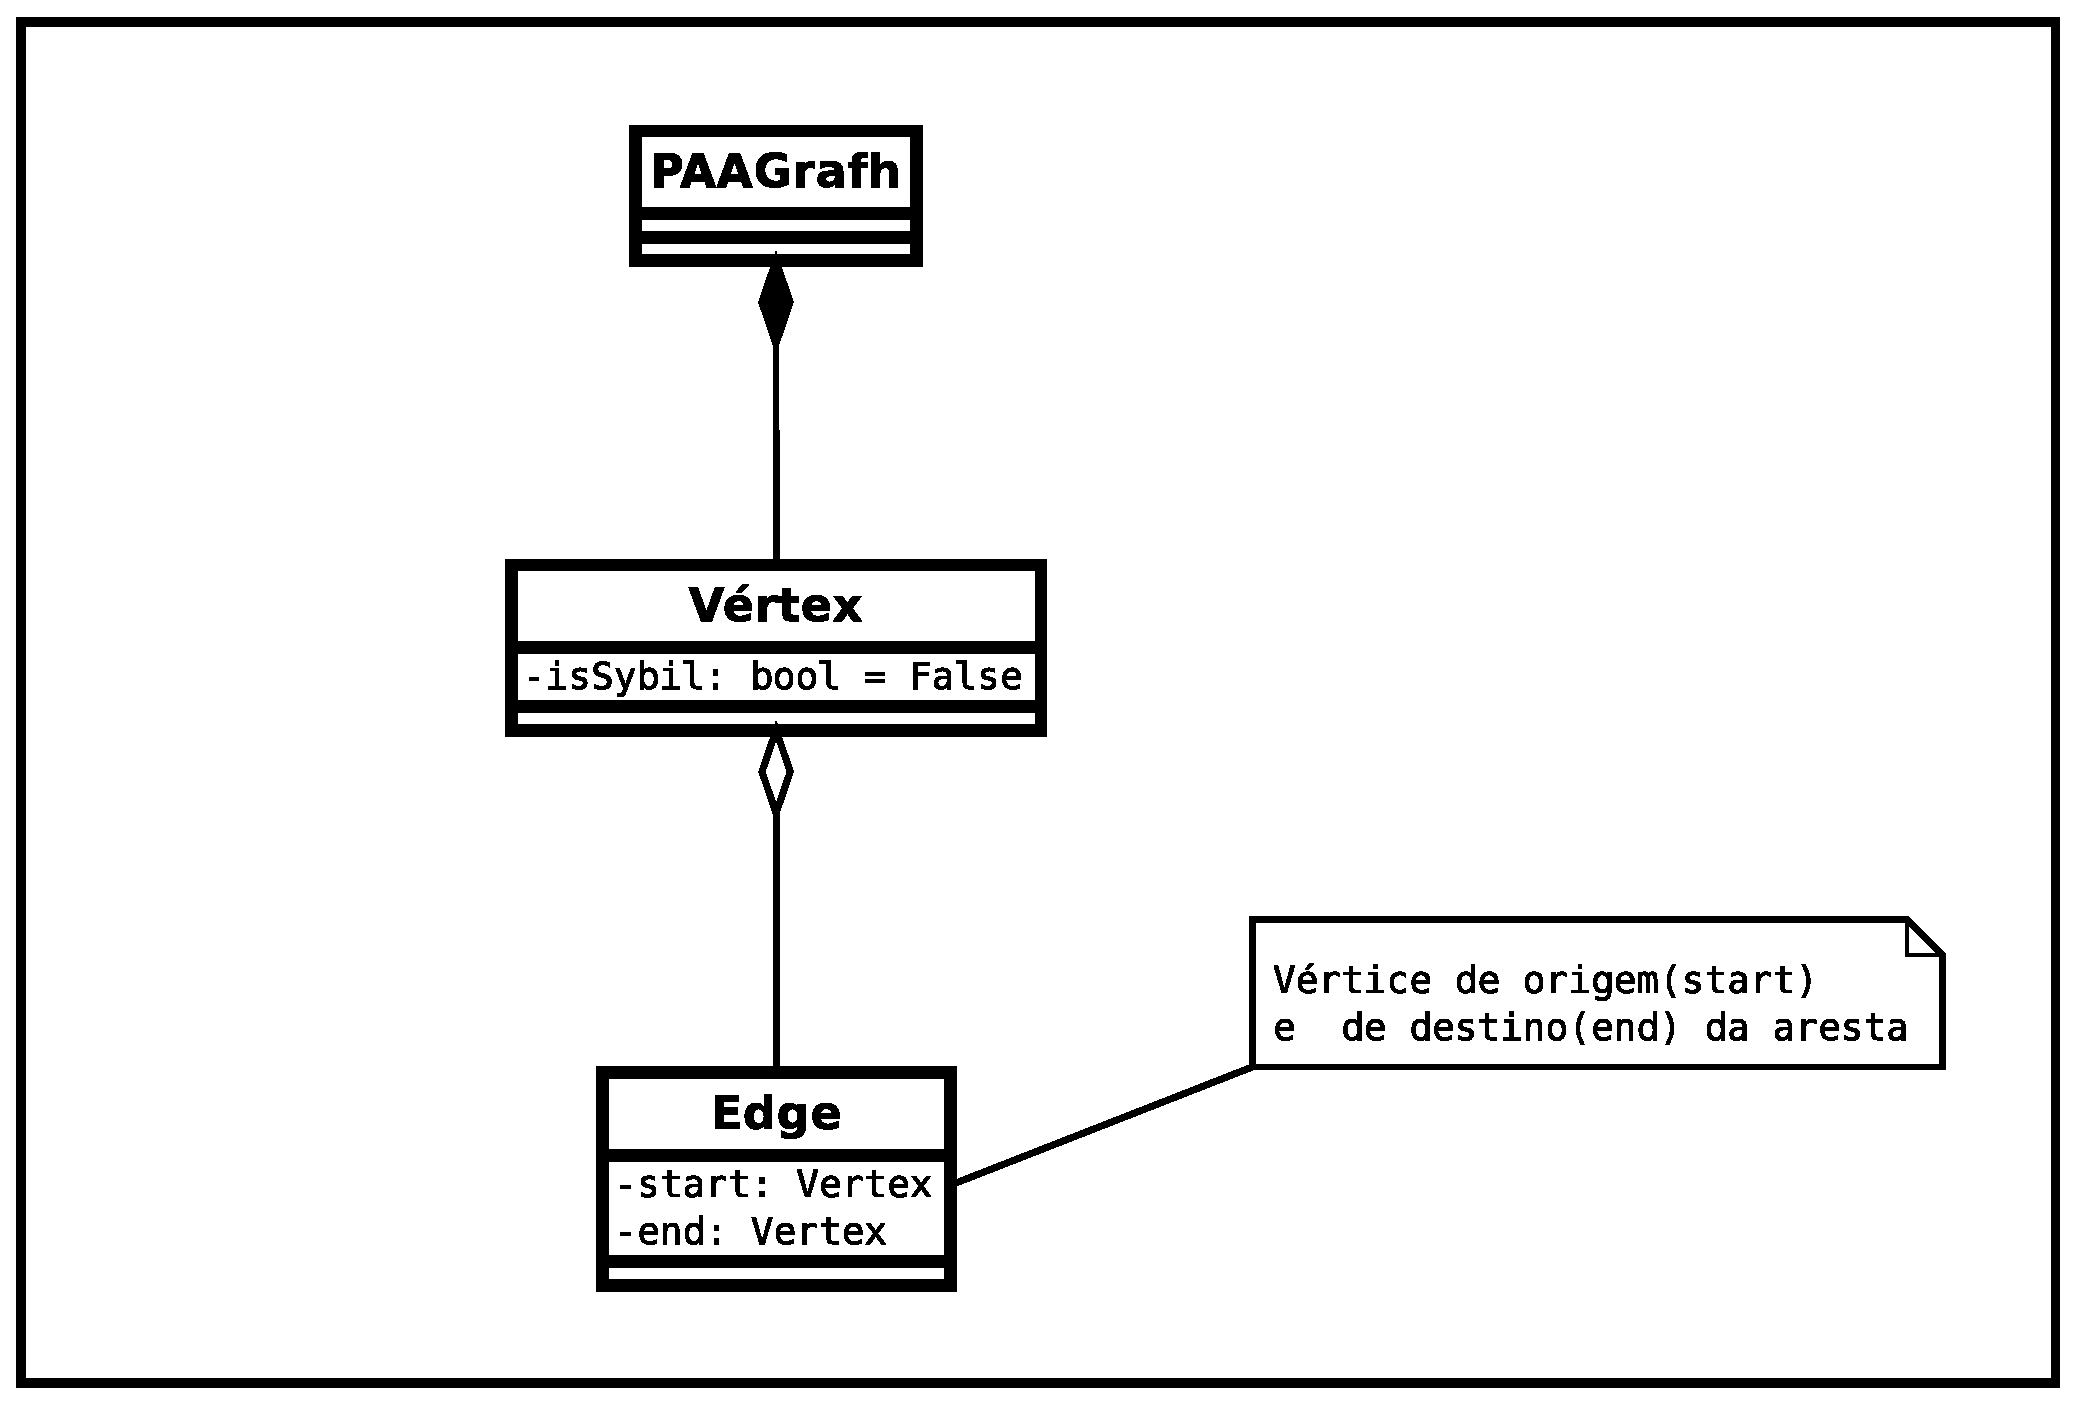
\includegraphics[width=0.7\textwidth]{../img/cd_graph.eps}
\caption{Diagrama de Classe de um Grafo}
\label{fig:cd_graph}
\end{figure}


Para cada vértice pertencente ao conjunto $V$ existe um atributo denominado \textit{isSybil} que determina se aquela vértice pertence à região \emph{honesta (A)} ou à região \emph{Sybil (B)}. Inicialmente todo os vértices são considerados como \textit{Sybil}, ou seja, $V = B$. Posteriormente, com base em informações previamente fornecidas, um total de $k$ vértice serão definidos como \textit{honestos}. Este conjunto $S \in V$ para o qual se sabe previamente serem honesto será denominado \textit{sementes}, e a partir destas sementes os demais vértices serão classificados. O processo de seleção das ``sementes" bem como da classificação dos vértices é detalhado na Subseção \ref{subsec:particao}{}.

\subsection{Particionamento do Grafo}
\label{subsec:particao}

Estudos vêm demonstrando que um possível mecanismo contra ataques é por meio da implementação de \textit{Algoritmo de Detecção de Comunidades (ADC)} \cite{viswanath2011analysis}. Este tipo de algoritmo consiste basicamente em identificar vértices formando uma comunidade local em torno de determinado vértice garantidamente honesto. Os demais vértices, que estão fora da comunidade, são considerados uma ameaça, e portanto classificados como \textit{Sybil}. Uma possível maneira de classifica uma comunidade é através de sua \textit{Condutância Normalizada}.

\subsubsection{Condutância Normalizada}
\label{subsubsec:condutancia_normalizada}

Neste trabalho, como técnica de detecção de comunidade utilizou-se o conceito de \textit{Condutância} de um Grafo, que é uma métrica que define a qualidade de uma única comunidade \cite{kannan2004clusterings}. A condutância de um grafo $G = (V, E)$, onde $A \in V$ e $B = V-A$ formam duas comunidades distintas é definido conforme a Equação \ref{eq:condutancia}, onde $e_{AB}$  é o número de aresta entre os vértice da comunidade $A$ e $B$ e $e_{AA}$ representa o número de aresta entre os vértices da comunidade $A$.

\begin{equation} \label{eq:condutancia}
C = \frac{e_{AB}}{e_{AA}} 
\end{equation}

No entanto, a definição de condutância conforme descrito na \ref{eq:condutancia} não é uma boa medida para a qualidade de uma comunidade, quando  se está analisando comunidades de tamanhos maiores \cite{mislove2010you}, como é caso em redes sociais. Por exemplo, caso todo os vértices fossem classificados em uma única comunidade, como por exemplo a região honesto, a condutância resultante seria igual a \textit{zero}, fornecendo poucas informações sobre a comunidade formada. Visando definir uma métrica aplicável em comunidades maiores foi proposto no trabalho de \cite{mislove2010you} a \textit{Condutância Normalizada} de um grafo.Para derivar a condutância normalizada, deve-se definir o valor $K$ de uma comunidade $A$ qualquer conforme Equação \ref{eq:valor_k}. O valor $k$  é similar à condutância, exceto por estar no intervalo $[0, 1]$. 

\begin{equation} \label{eq:valor_k}
K = \frac{e_{AA}}{e_{AA} + e_{AB}} 
\end{equation}

A Condutância Normalizada $CN$ de uma comunidade $A$ é como $K$ menos o valor esperado de $K$ para um grafo particionado em comunidades de tamanho $|A|$ e $|B|$. Para calcular o valor esperado de $K$, é necessário calcular o valor esperado de $e_{AA}$ e $e_{AB}$ mas sem levar em conta as arestas das comunidades.
Desse modo, a Condutância Normalizada $CN$ é definida conforme a Equação \ref{eq:condutancia_normalizada}, onde $e_A= e_{AA} + e_{AB}$ que determina o número de aresta que alcançam os vértices na comunidade $A$ e $e_B = e_{BB} + e_{AB}$ representa a mesma quantidade para a comunidade $B$.

\begin{equation} \label{eq:condutancia_normalizada}
CN = \frac{e_{AA}}{e_{AA} + e_{AB}}  - \frac{e_A \times e_B}{e_A \times e_A + e_A \times e_B}
\end{equation}

Os valores de $CN$ estão definidos no intervalo $[-1,1]$ onde \textit{valores positivos} indicam uma estrutura de comunidade significativa; um valor \textit{0 (zero)} indica que não há uma estrutura de comunidade, e um \textit{valor negativo} indica que a estrutura de comunidade é menor do que a de um
grafo aleatório. Uma propriedade particularmente útil dessa definição é que ela é comparável entre grafos de tamanhos e densidades diferentes.

A partir dos valores calculados de $CN$ é possível particionar um grafo em uma região honesta (comunidade A) e região Sybil (comunidade B). A ideia básica é definir uma comunidade inicial $A$ em que inicialmente todos os vértices são garantidamente honesto e permitir a inclusão de um vértice $v$ na comunidade $A$ apenas se a inclusão de $v$ aumentar a \textit{Condutância Normalizada} de $A$.  O algoritmo guloso que particiona um grafo com base na \textit{Condutância Normalizada} é descrito na Subseção \ref{subsubsec:algoritmo}.

\subsubsection{Algoritmo Guloso para Particionamento de um Grafo}
\label{subsubsec:algoritmo}

Suponha que nos seja dado um grafo $G(V,E)$ para o qual se deseja particioná-lo em duas regiões $A$ e $B$. A região $A$ representa os vértices dito \textit{honestos} e a região $B$ conterá os vértices classificados como \textit{Sybil}. Suponha ainda que conheçamos previamente que exista um conjunto $ H \in V$ de vértices \textit{garantidamente} honestos. A partir do conjunto $H$ é definido um subconjunto $S \in H$ escolhidos aleatoriamente de forma a produzir inicialmente o conjunto $A$. 


Procedendo conforme descrito no parágrafo anterior, o G é dividido em duas partições $A$ e $B$, inicialmente com $A = S$ e $B = (V-S)$. A cada passo, é selecionado um vértice $v \in B$ ao \textit{apenas será adicionado ao conjunto $A$ caso $v$ produza um aumento no valor $CN$ de $A$}. Esse processo se repete adicionando vértices em $A$ até que não reste nenhum vértice que aumente o valor de $CN$ . Então, o algoritmo pára e retorna como saída a comunidade $A$ definida como a região honesta. De forma análoga, $B = (V-A)$ será considerada como a região Sybil. O Algoritmo \ref{algo:guloso_adc} demonstra todos os passos deste processo.

Conforme pode ser observado o algoritmo escolhe de forma aleatória um conjunto de sementes $S$ (\textit{linha 7}. Este conjunto se torna inicialmente o conjunto honesto $A$ (\textit{linha 8}). Posteriormente os demais vértices $V-S$ são adicionados a uma fila $Q$ e serão inseridos nos conjuntos $A$ ou $B$ (\textit{linhas 11 a 19}). Em suma, um vértice é inicialmente definido como honesto (\textit{linha 13}), caso esta suposição aumento o valor $CN$ do grafo (\textit{linha 15}) o vértice é mantido em $A$. Do contrário ele é removido e adicionado em $B$ (\textit{linhas 18 e 19}). O algoritmo termina quando fila $Q$ estiver vazia.

O tempo de execução do Algoritmo \ref{algo:guloso_adc} dependerá basicamente do tamanho do conjunto $S$ e da função \textsc{CALCULE-CN}. A seção \ref{sec:analise_complexidade} discutirá com mais detalhes a complexidade de tempo e de espaço do algoritmo. Contudo, podemos ressaltar neste ponto que $|H| = 100$ e $|S| = 20$, ou seja, para cada grafo analisado foi definido inicialmente um total de $100$ vértices honestos, deste total $20$ são escolhidos randomicamente para ser as sementes do conjunto $A$.


\begin{algorithm}
\SetKwFunction{CHOOSERANDOMSEED}{CHOOSE-RANDOM-SEED}
\SetKwFunction{CALCULECN}{CALCULE-CN}
\SetKwFunction{DEQUEUE}{DEQUEUE}
\DontPrintSemicolon % Some LaTeX compilers require you to use \dontprintsemicolon instead
\KwIn{Um grafo $G(V,A)$ e um conjunto de vértices $H \in V$ definidos como honestos}
\KwOut{Os subconjuntos $A, B \in V$ tal que $A \cap B = \emptyset$, onde $A$ contêm os vértices classificados
como honesto e $B$ os vértices classificados como Sybil}

$A \gets \emptyset$\;
$B \gets \emptyset$\;
$Q \gets \emptyset$\;
$S \gets \emptyset$\;
$CN_{current} \gets 0$\;
$CN_{new} \gets 0$\;

$S \gets$ \CHOOSERANDOMSEED{$H$}\;

$A \gets S$\;
$Q \gets (V-S)$\;

$CN_{current} \gets$ \CALCULECN{$G(V,E)$}\;


\While{$Q \neq \emptyset$} {

	$v \gets$ \DEQUEUE{$Q$}\;
	$A \gets A \cup v$\;
	
	$CN_{new} \gets$ \CALCULECN{$G(V,E)$}\;
	
	\If{$CN_{new} \geq CN_{current}$}{
			
		$CN_{current} \gets CN_{new}$\;		
	
	}\Else{
	
		$A \gets A - v$\;
		$B \gets B \cup v$\;	
	}
    
}
\Return{$A,B$}\;
\caption{\sc Algoritmo Guloso para definição de Sybil's em um grafo.}
\label{algo:guloso_adc}
\end{algorithm}

\subsection{Cálculo das Métricas}
\label{subsec:metricas}

Com o objetivo de mensurar a qualidade dos resultados obtidos pelo algoritmo proposto neste trabalho, foi utilizado um conjunto dez métricas. A partir destas métricas é possível comparar a qualidade da resposta obtida bem como verificar o comportamento do algoritmo para grafos de diferentes estruturas. As métricas utilizadas são:

\begin{enumerate}[(a)]
	\item grau médio dos vértices:
	\item modularidade\footnote{Conforme proposto em \cite{mislove2010you}}
	\item condutância da região Sybil
	\item condutância da região honesta
	\item coeficiente de agrupamento da região Sybil
	\item coeficiente de agrupamento da região honesta
	\item fração de vértices Sybil corretamente classificados;
	\item fração de vértices honestos corretamente classificados
	\item fração de falsos positivos
	\item fração de falsos negativos
de forma incorreta como honestos).
\end{enumerate}


\section{Análise de Complexidade}
\label{sec:analise_complexidade}

\subsection{Complexidade Temporal}
\label{subsec:complex_temporal}

Conforme discutido anteriormente o principal algoritmo proposto neste trabalho é aquele descrito no pseudocódigo do Algoritmo \ref{algo:guloso_adc}{}. Aquele algoritmo dependerá basicamente do tamanho do conjunto de sementes $S$ e do tempo de execução dos métodos \textsc{CHOOSE-RANDOM-SEED} e \textsc{CALCULE-CN}.

A função \textsc{CHOOSE-RANDOM-SEED} têm como objetivo escolher randomicamente $|S|$ vértices em um conjunto de tamanho $|H|$. Esta escolha pode ser feita no pior caso em tempo linear ao tamanho do conjunto $H$. Desta forma a complexidade de tempo do método \textsc{CHOOSE-RANDOM-SEED} pode ser definida como $O(H)$;

A \textit{Condutância Normalizada} obtida através do método \textsc{CALCULE-CN} é calculada avaliando cada uma das arestas dos vértices em $V$. Neste sentido, no pior caso, a complexidade de tempo da função \textsc{CALCULE-CN} será dada por $O(V \times A)$. Contudo, conforme pode ser observado na \textit{linha 14} do Algoritmo \ref{algo:guloso_adc}, o método \textsc{CALCULE-CN} será executado $|V-S|$ vezes. Neste sentido, a participação de \textsc{CALCULE-CN} na complexidade do algoritmo \ref{algo:guloso_adc} será de $ (V-S) \times V \times A$. Contudo, se consideramos que $S \ll V$ a complexidade de tempo do Algoritmo \ref{algo:guloso_adc} será dada por $O(V^{2} \times A)$.

\subsection{Complexidade Espacial}
\label{subsec:complex_espacial}

A Subseção \ref{subsec:modelagem} descreveu que neste trabalho foi utilizado uma representação de grafo onde cada vértice armazena um conjunto de suas sua arestas (vide Figura \ref{fig:cd_graph}). Partindo desta premissa a \textit{Complexidade de Espaço} do algoritmo será de $O(V+A)$, ao qual se refere-se no espaço necessário para armazenar os $|V|$ vértice e as $|A|$ arestas. Haverá a necessidade de armazenar os conjuntos $A$ e $B$, contudo, como $ A \cup B = V$, assintoticamente não mudaria o valor da complexidade de espaço do algoritmo.	

\section{Análise Experimental}
\label{sec:experimentos}

Com o objetivo de verificar a qualidade das respostas dadas pelo algoritmo foi recuperado o conjunto de métricas descritos na Subseção \ref{subsec:metricas}. Os testes consistem em executar o algoritmo por \textit{100} vezes para cada um dos grafos de entrada. Esse procedimento é necessário tendo em vista a escolha aleatória das sementes. Os testes foram executados em computador com o sistema operacional Ubuntu versão 12.04 kernel 3.13.0-37-generic 64 bits e com 4GB de memória RAM. O valor médio para cada uma das execuções estão exibidos nas Tabelas \ref{tab:metricas_parte_01}{} e \ref{tab:metricas_parte_02}{}

% Please add the following required packages to your document preamble:
% \usepackage{multirow}
% \usepackage{graphicx}
% \usepackage[table,xcdraw]{xcolor}
% If you use beamer only pass "xcolor=table" option, i.e. \documentclass[xcolor=table]{beamer}
\begin{table}[h]
\centering
\resizebox{\textwidth}{!}{%
\begin{tabular}{|c|c|c|c|c|}
\hline
\rowcolor[HTML]{C0C0C0} 
\cellcolor[HTML]{C0C0C0}                              & \multicolumn{4}{c|}{\cellcolor[HTML]{C0C0C0}{\bf MÉTRICAS}}                                              \\ \cline{2-5} 
\rowcolor[HTML]{C0C0C0} 
\multirow{-2}{*}{\cellcolor[HTML]{C0C0C0}{\bf GRAFO}} & {\bf grau médio dos vértices} & {\bf modularidade} & {\bf Condutância Sybil} & {\bf Condutância Honesta} \\ \hline
{\bf A}                                               & 15.7708                       & 0,825              & 14765.7                 & 16276.9                   \\ \hline
{\bf B}                                               & 15.9552                       & 0.899              & 16135                   & 12504.3                   \\ \hline
\end{tabular}
}
\caption{Métricas Grafos A e B - Parte 01/02}
\label{tab:metricas_parte_01}
\end{table}

É possível verificar que mesmo para grafos de estrutura diferentes (Grafo A e B) o algoritmo apresentou resultando semelhantes mostrando que o uso da \textit{Condutância Normalizada} conseguiu melhorar a qualidade dos resultados independente do tamanho e estrutura das comunidades existentes nos grafos.

% Please add the following required packages to your document preamble:
% \usepackage{multirow}
% \usepackage{graphicx}
% \usepackage[table,xcdraw]{xcolor}
% If you use beamer only pass "xcolor=table" option, i.e. \documentclass[xcolor=table]{beamer}
\begin{table}[h]
\centering
\resizebox{\textwidth}{!}{%
\begin{tabular}{|c|c|c|c|c|c|c|}
\hline
\rowcolor[HTML]{C0C0C0} 
\cellcolor[HTML]{C0C0C0}                              & \multicolumn{6}{c|}{\cellcolor[HTML]{C0C0C0}{\bf MÉTRICAS}}                                                                                            \\ \cline{2-7} 
\rowcolor[HTML]{C0C0C0} 
\multirow{-2}{*}{\cellcolor[HTML]{C0C0C0}{\bf GRAFO}} & {\bf Coef. Agrup Sybil} & {\bf Coef. Agrup Honesto} & {\bf Sybil Corretos} & {\bf Honestos Corretos} & {\bf falsos positivos} & {\bf falsos negativos} \\ \hline
{\bf A}                                               & 0.0912714               & 0.0959462                 & 1                    & 0,09766                 & 0.474333               & 0                      \\ \hline
{\bf B}                                               & 0.0891779               & 0.0937305                 & 1                    & 0.86                    & 0.122807               & 0                      \\ \hline
\end{tabular}
}
\caption{Métricas Grafos A e B - Parte 02/02}
\label{tab:metricas_parte_02}
\end{table}


\section{Conclusão}
\label{sec:conclusao}

Este trabalho resolver o problema de particionar um grafo em duas em duas regiões, a região \emph{honesta (A)} e a região \emph{Sybil (B)}. Utilizando um algoritmo guloso que faz uso da métrica \textit{Condutância Normalizada} foi possível detectar de forma satisfatória vértices como Sybil. O fato de utilizar a Condutância Normalizada possibilitou a aplicação do algoritmo em grafos de diferente estrutura e tamanhos, obtendo resultados semelhantes para cada um deles.

\bibliographystyle{sbc}
\bibliography{sbc-template}

\end{document}
